% Template GRASS newsletter - Article
% Language: Latex
%

% Head
\graphicspath{{./images/}}

\title{Starter Manual to GRASS GIS}
\subtitle{GRASS Original}
\author{GRASS Development Team}

\maketitle

\section{Introduction}

This screenshot is GRASS GIS running on Ubuntu, it does seamlessly in MacOSX and Windows too.Fig.~\ref{fig:grass000}
%\setkeys{Gin}{width=1\textwidth}
\begin{figure}[htbp]
   \centering
   %name of your graphic, without the path AND in PNG (screnshots etc)/PDF (drawings) format:
   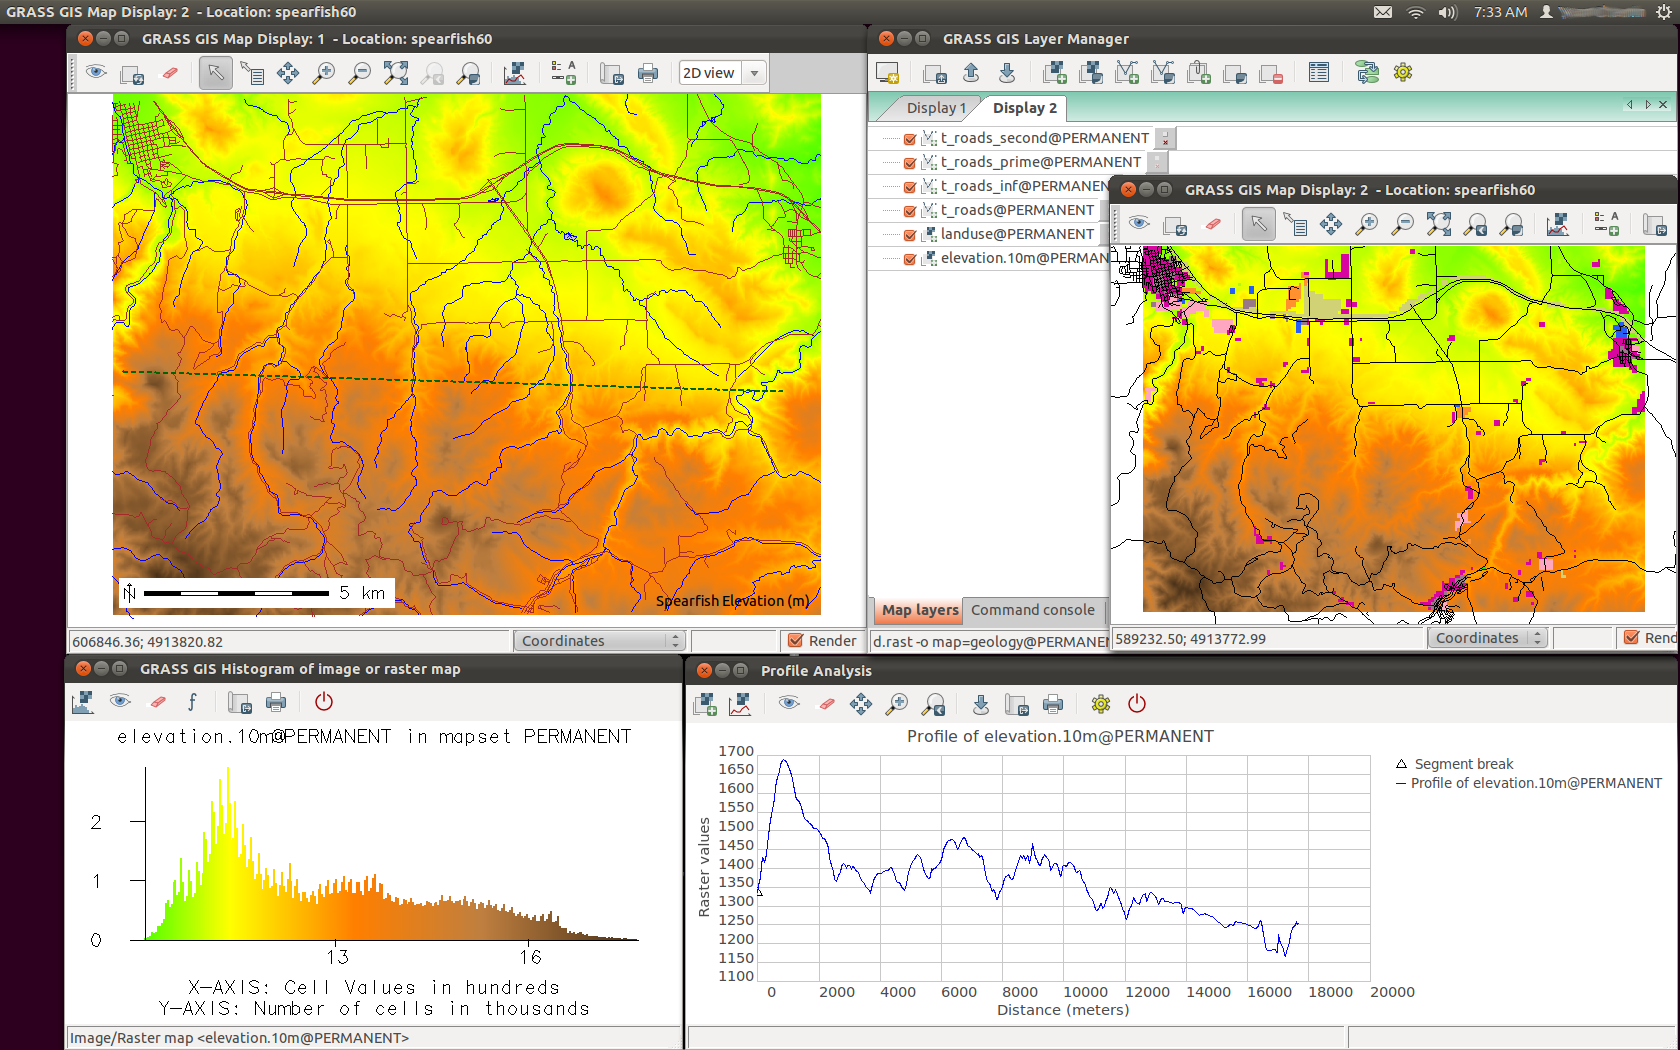
\includegraphics[scale=0.125]{grass000.png}
   %caption of the figure
   \caption{GRASS on Ubuntu}
   %label of the figure, which has to correspond to \ref{}:
   \label{fig:grass000}
\end{figure}

Starting GRASS GIS: Select Spearfish60 Location by a click on
``Enter GRASS'':Fig.~\ref{fig:grass001}

%\setkeys{Gin}{width=1\textwidth}
\begin{figure}[htbp]
   \centering
   %name of your graphic, without the path AND in PNG (screnshots etc)/PDF (drawings) format:
   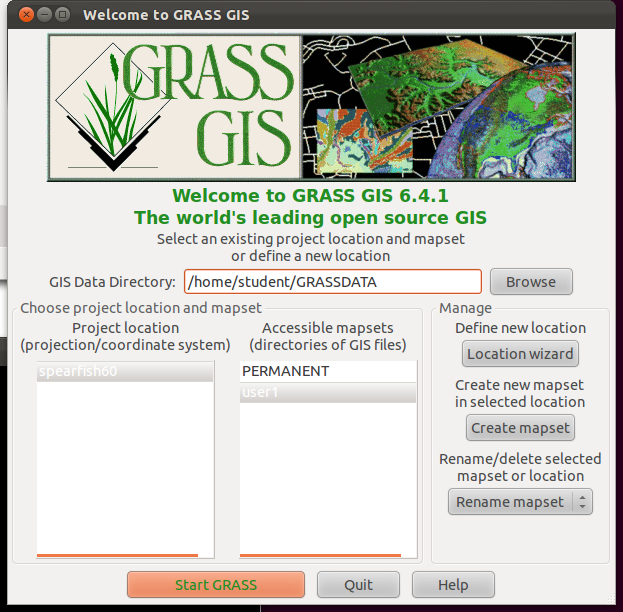
\includegraphics[scale=0.4]{grass001.png}
   %caption of the figure
   \caption{Welcome Screen}
   %label of the figure, which has to correspond to \ref{}:
   \label{fig:grass001}
\end{figure}

At this point it should (somewhat) look this way: Fig.~\ref{fig:grass002}

%\setkeys{Gin}{width=1\textwidth}
\begin{figure}[htbp]
   \centering
   %name of your graphic, without the path AND in PNG (screnshots etc)/PDF (drawings) format:
   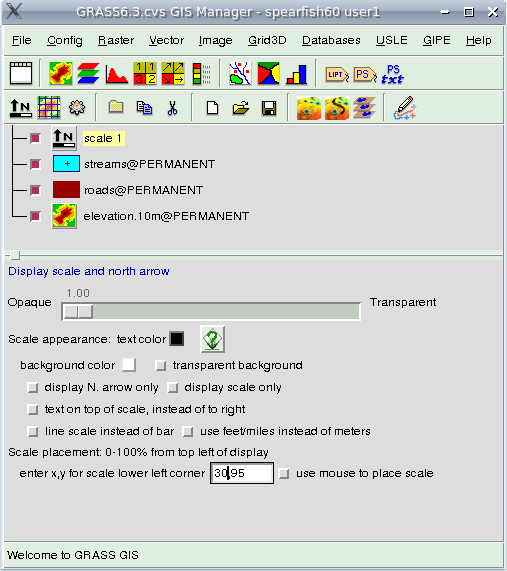
\includegraphics[scale=0.35]{grass002.png}
   %caption of the figure
   \caption{GIS Manager}
   %label of the figure, which has to correspond to \ref{}:
   \label{fig:grass002}
\end{figure}

Some more GRASS GUI information is found in Appendix A \ref{appendixA}.

Load the elevation.10m layer by clicking on the raster display button
(fifth button from left):Fig.~\ref{fig:grass003}

%\setkeys{Gin}{width=1\textwidth}
\begin{figure}[htbp]
   \centering
   %name of your graphic, without the path AND in PNG (screnshots etc)/PDF (drawings) format:
   
\includegraphics[scale=0.5]{grass003.png}
   %caption of the figure
   \caption{Basic Display}
   %label of the figure, which has to correspond to \ref{}:
   \label{fig:grass003}
\end{figure}

Once selected, the main GRASS GUI will have a new layer like one of
these in Fig.~\ref{fig:grass004}

%\setkeys{Gin}{width=1\textwidth}
\begin{figure}[htbp]
   \centering
   %name of your graphic, without the path AND in PNG (screnshots etc)/PDF (drawings) format:
   
\includegraphics[scale=0.5]{grass004.png}
   %caption of the figure
   \caption{}
   %label of the figure, which has to correspond to \ref{}:
   \label{fig:grass004}
\end{figure}

By selecting the new layer, you will be given a contextual menu below:Fig.~\ref{fig:grass005}

%\setkeys{Gin}{width=1\textwidth}
\begin{figure}[htbp]
   \centering
   %name of your graphic, without the path AND in PNG (screnshots etc)/PDF (drawings) format:
   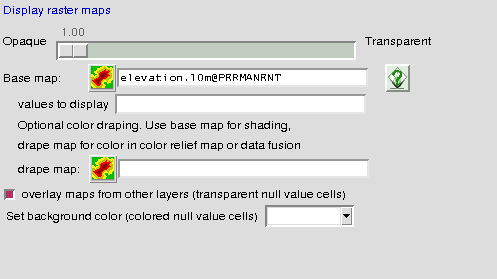
\includegraphics[scale=0.35]{grass005.png}
   %caption of the figure
   \caption{}
   %label of the figure, which has to correspond to \ref{}:
   \label{fig:grass005}
\end{figure}

Then add a vector using the 7th icon from the left. Fig.~\ref{fig:grass006}

%\setkeys{Gin}{width=1\textwidth}
\begin{figure}[htbp]
   \centering
   %name of your graphic, without the path AND in PNG (screnshots etc)/PDF (drawings) format:
   
\includegraphics[scale=0.5]{grass006.png}
   %caption of the figure
   \caption{}
   %label of the figure, which has to correspond to \ref{}:
   \label{fig:grass006}
\end{figure}

Add a stream layer (blue color) and a road layer (brown color). Below is
the example for the streams Fig.~\ref{fig:grass007}

%\setkeys{Gin}{width=1\textwidth}
\begin{figure}[htbp]
   \centering
   %name of your graphic, without the path AND in PNG (screnshots etc)/PDF (drawings) format:
   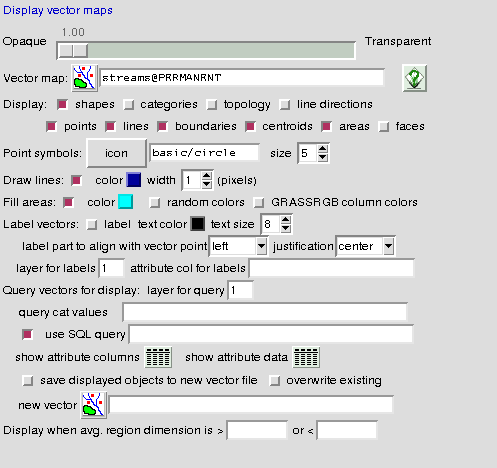
\includegraphics[scale=0.45]{grass007.png}
   %caption of the figure
   \caption{}
   %label of the figure, which has to correspond to \ref{}:
   \label{fig:grass007}
\end{figure}

Result should look like this (somehow):Fig.~\ref{fig:grass008}

%\setkeys{Gin}{width=1\textwidth}
\begin{figure}[htbp]
   \centering
   %name of your graphic, without the path AND in PNG (screnshots etc)/PDF (drawings) format:
   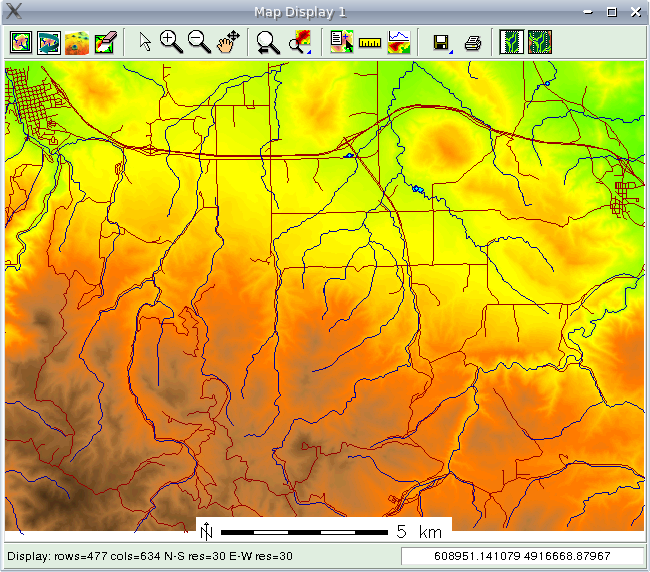
\includegraphics[scale=0.35]{grass008.png}
   %caption of the figure
   \caption{}
   %label of the figure, which has to correspond to \ref{}:
   \label{fig:grass008}
\end{figure}

\section{DEM MANIPULATIONS}
Remove the vector layers from the display, and the annotations too. Display only an elevation map as in Fig.~\ref{fig:grass009}

%\setkeys{Gin}{width=1\textwidth}
\begin{figure}[htbp]
   \centering
   %name of your graphic, without the path AND in PNG (screnshots etc)/PDF (drawings) format:
   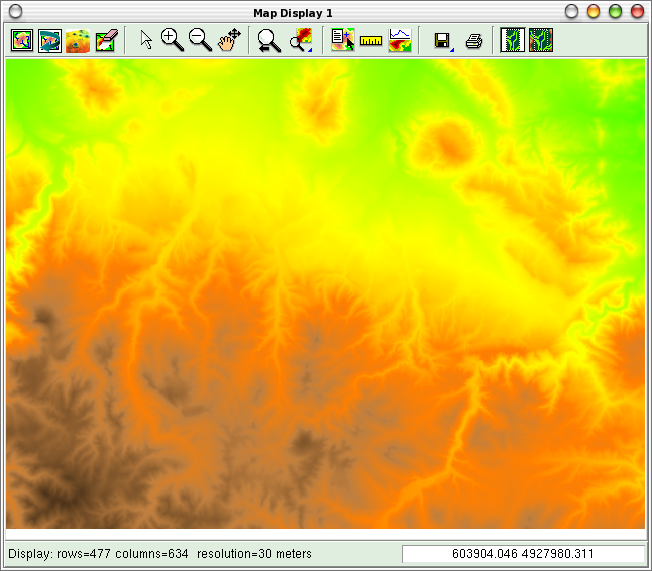
\includegraphics[scale=0.35]{grass009.png}
   %caption of the figure
   \caption{Display a DEM}
   %label of the figure, which has to correspond to \ref{}:
   \label{fig:grass009}
\end{figure}

\subsection{Compute slope and aspect}
Raster/Terrain Analysis/Slope and Aspect. Fig.~\ref{fig:grass010}

%\setkeys{Gin}{width=1\textwidth}
\begin{figure}[htbp]
   \centering
   %name of your graphic, without the path AND in PNG (screnshots etc)/PDF (drawings) format:
   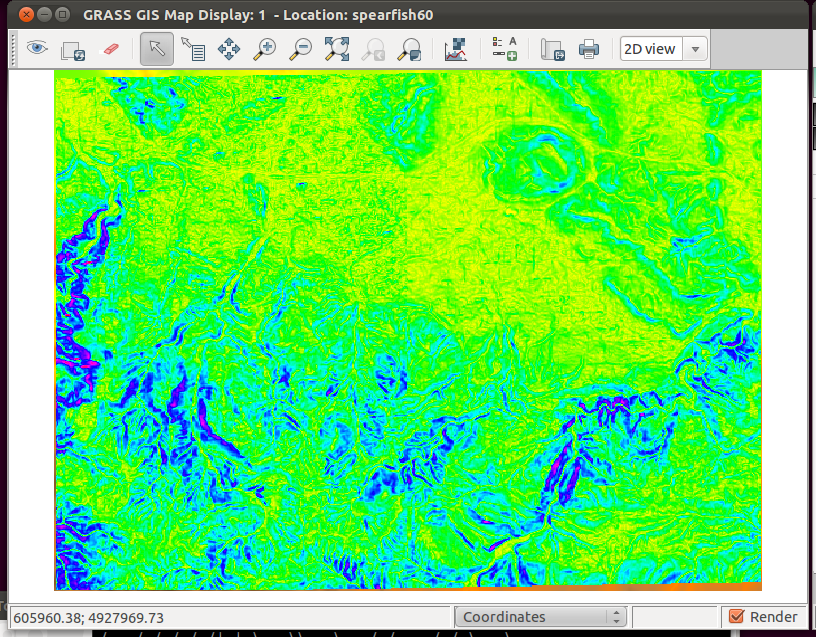
\includegraphics[scale=0.35]{grass010.png}
   %caption of the figure
   \caption{Slope}
   %label of the figure, which has to correspond to \ref{}:
   \label{fig:grass010}
\end{figure}

Compute a shaded relief map ( in Raster/Terrain Analysis/Shaded Relief).
The Shaded Relief map should be like this when a elevation.10m map is overlaid to it with 0.5 opacity (right-click on elevation.10m layer and change opacity level): Fig.~\ref{fig:grass011}

%\setkeys{Gin}{width=1\textwidth}
\begin{figure}[htbp]
   \centering
   %name of your graphic, without the path AND in PNG (screnshots etc)/PDF (drawings) format:
   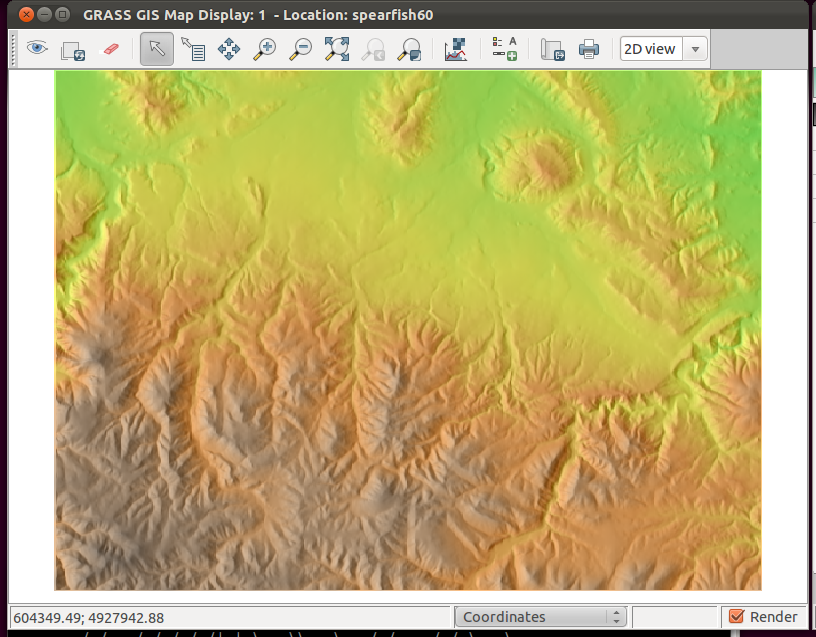
\includegraphics[scale=0.35]{grass011.png}
   %caption of the figure
   \caption{Shaded Relief}
   %label of the figure, which has to correspond to \ref{}:
   \label{fig:grass011}
\end{figure}

\subsection{Watershed Basin Analysis Program}
Raster/Hydrologic modeling/Watershed Analysis.
Fill in the Elevation input map with ``elevation.10m''. The minimum size of an exterior watershed basin should be 5000 cells. Fill up output names for all the output maps available (i.e. ``\_cells\_nbr'', ``\_drain\_dir'', ``\_basins'', ``\_streams'', ``\_half\_basins'', ``\_visual'', ``\_LS'', ``\_S'').

Output should state the following:

SECTION 1a (of 6): Initiating Memory.

SECTION 1b (of 6): Determining Offmap Flow.

SECTION 2: A * Search.

SECTION 3: Accumulating Surface Flow.

SECTION 4: Length Slope determination.

SECTION 5: Watershed determination.

SECTION 6: Closing Maps.

Output of ``\_basins'' should look like this:Fig.~\ref{fig:grass012}

%\setkeys{Gin}{width=1\textwidth}
\begin{figure}[htbp]
   \centering
   %name of your graphic, without the path AND in PNG (screnshots etc)/PDF (drawings) format:
   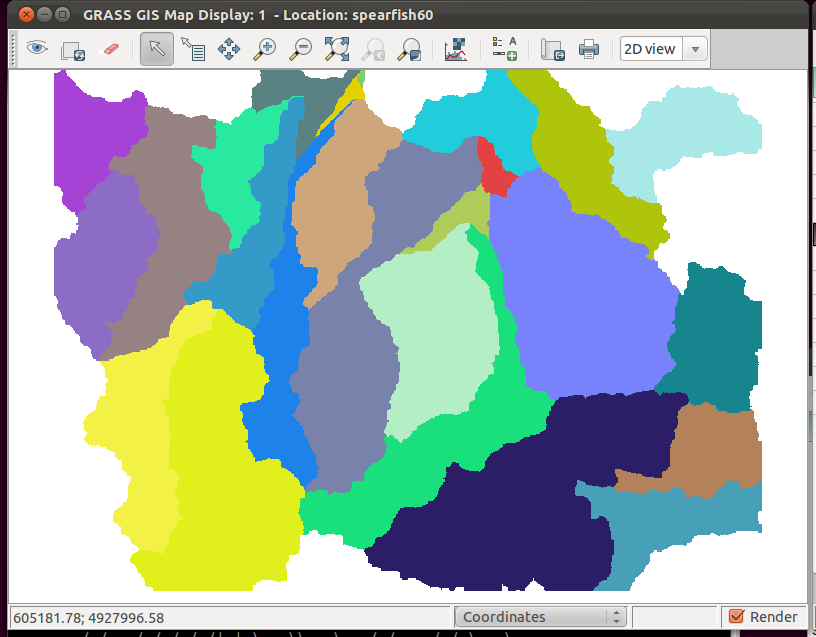
\includegraphics[scale=0.35]{grass012.png}
   %caption of the figure
   \caption{Generated Basins}
   %label of the figure, which has to correspond to \ref{}:
   \label{fig:grass012}
\end{figure}


Output of ``\_streams'' should look like this: Fig.~\ref{fig:grass013} compare it with
the vector map ``streams''.

%\setkeys{Gin}{width=1\textwidth}
\begin{figure}[htbp]
   \centering
   %name of your graphic, without the path AND in PNG (screnshots etc)/PDF (drawings) format:
   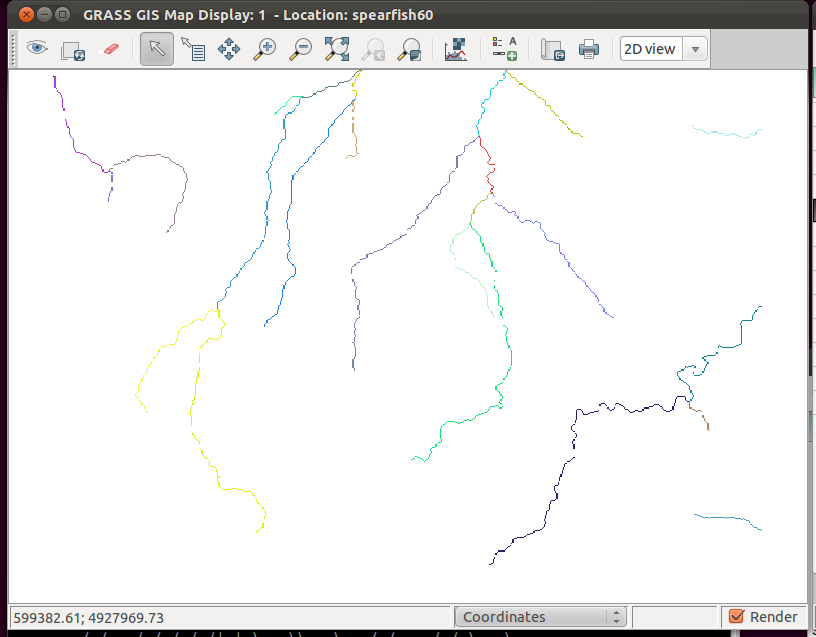
\includegraphics[scale=0.35]{grass013.png}
   %caption of the figure
   \caption{Generated streams}
   %label of the figure, which has to correspond to \ref{}:
   \label{fig:grass013}
\end{figure}

Relaunch with various values instead of 5000 cells, i.e. 2000 and 10000.
Compare by vectorizing the streams generated. Vectorization follows
these steps:\newline
1-Raster/Transform Features/Thin\newline
2-File/Map Type Conversion/Raster to Vector Map\newline
3-Vector/Develop Vector Map/Create or Rebuild Topology (optional)\newline

\subsection{Stream Pollution Monitoring Station site identification}
Assuming a Wood Processing Factory is requesting permit to setup a new processing plant in the country side. It is remote from major mapped streams (598713.35(E) 4920069.15(N)), the local council gave you a notice to assess the path of some minor effluents that may be draining to the major stream from the future factory, and especially their meeting point coordinates where the council will establish an automatic monitoring station.
Use Raster/Terrain Analysis/Least Cost Route Or Flow, your output should look like this: Fig.~\ref{fig:grass014}

%\setkeys{Gin}{width=1\textwidth}
\begin{figure}[htbp]
   \centering
   %name of your graphic, without the path AND in PNG (screnshots etc)/PDF (drawings) format:
   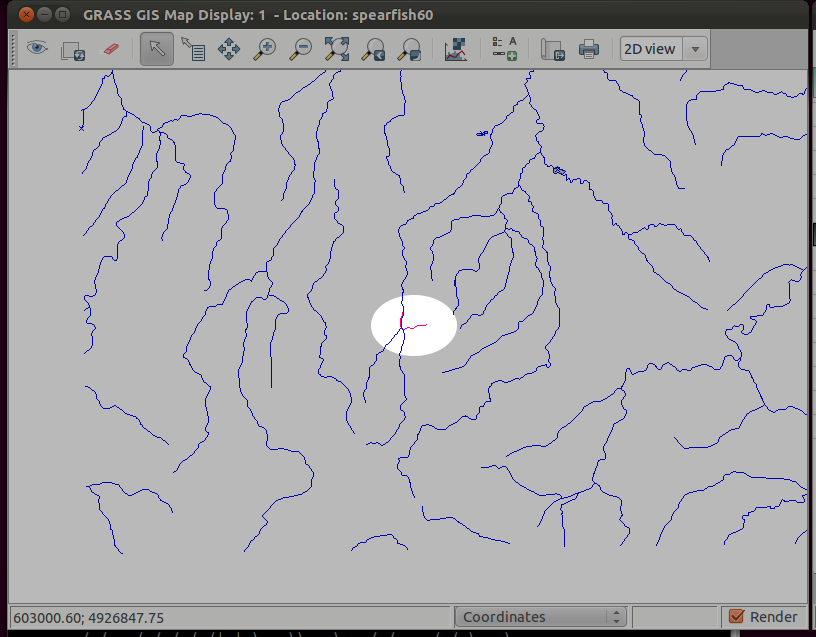
\includegraphics[scale=0.35]{grass014.png}
   %caption of the figure
   \caption{}
   %label of the figure, which has to correspond to \ref{}:
   \label{fig:grass014}
\end{figure}

What is the location (Easting,Northing) of the generated stream crossing
the mapped stream where it is proposed to install a monitoring
station?

\section{GRASS GIS Habitat Analysis}
\subsection{Introduction}

http://www.udel.edu/johnmack/frec682/682proj2.html

This course is available online under the course name ``FREC 682 Spatial Analysis''. This material is a modified version to accommodate with GRASS 6.4.1+.

In this session, the features needed are the following essentially (look in RASTER from the main interface):
The BUFFERING Module:   Raster/Create buffers Fig.~\ref{fig:grass015}
The MAP CALCULATOR Module:   Raster/Map Calculator Fig.~\ref{fig:grass016}

%\setkeys{Gin}{width=1\textwidth}
\begin{figure}[htbp]
   \centering
   %name of your graphic, without the path AND in PNG (screnshots etc)/PDF (drawings) format:
   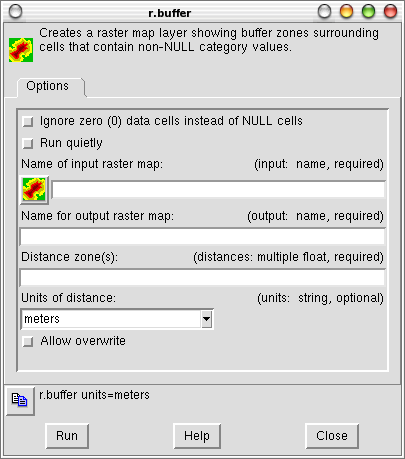
\includegraphics[scale=0.35]{grass015.png}
   %caption of the figure
   \caption{BUFFERING}
   %label of the figure, which has to correspond to \ref{}:
   \label{fig:grass015}
\end{figure}

%\setkeys{Gin}{width=1\textwidth}
\begin{figure}[htbp]
   \centering
   %name of your graphic, without the path AND in PNG (screnshots etc)/PDF (drawings) format:
   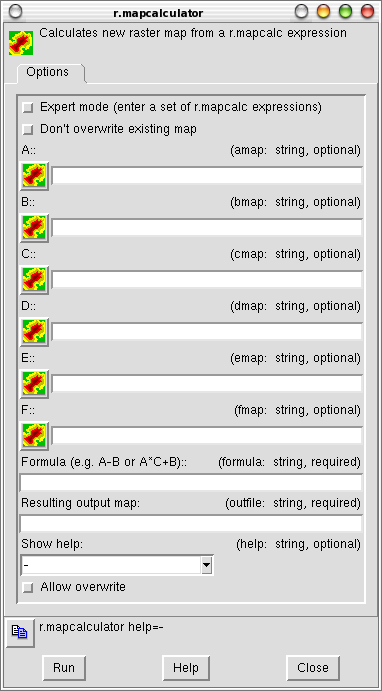
\includegraphics[scale=0.35]{grass016.png}
   %caption of the figure
   \caption{MAP CALCULATOR}
   %label of the figure, which has to correspond to \ref{}:
   \label{fig:grass016}
\end{figure}

Additional modules for the later part of the lab

Query map with mouse:
In the Map display window, look for:   Fig.~\ref{fig:grass017}

%\setkeys{Gin}{width=1\textwidth}
\begin{figure}[htbp]
   \centering
   %name of your graphic, without the path AND in PNG (screnshots etc)/PDF (drawings) format:
   
\includegraphics[scale=1]{grass017.png}
   %caption of the figure
   \caption{Query Map with mouse}
   %label of the figure, which has to correspond to \ref{}:
   \label{fig:grass017}
\end{figure}

\textbf{NULL values:}\newline Raster/Develop raster Map/Manage Null values\newline
\textbf{CLUMP:}\newline Raster/Transform features/Clump\newline
\textbf{STATISTICS:}\newline Raster/Reports \& Statistics/General statistics\newline
\textbf{R2V:}\newline File/Map type Conversions/Raster to vector\newline
\textbf{Vector Build:}\newline Vector/Develop Map/Create or Rebuild Topology\newline
\textbf{Vector Export:}\newline File/Export/Vector map/Common export formats\newline
\textbf{Start New Display Window:}\newline
In the main GRASS GUI look for:    Fig.~\ref{fig:grass018}

%\setkeys{Gin}{width=1\textwidth}
\begin{figure}[htbp]
   \centering
   %name of your graphic, without the path AND in PNG (screnshots etc)/PDF (drawings) format:
   
\includegraphics[scale=1]{grass018.png}
   %caption of the figure
   \caption{Launch New Display}
   %label of the figure, which has to correspond to \ref{}:
   \label{fig:grass018}
\end{figure}

Erase Display:
In the Map display window, look for:   Fig.~\ref{fig:grass019}

%\setkeys{Gin}{width=1\textwidth}
\begin{figure}[htbp]
   \centering
   %name of your graphic, without the path AND in PNG (screnshots etc)/PDF (drawings) format:
   
\includegraphics[scale=1]{grass019.png}
   %caption of the figure
   \caption{Erase Display Icon}
   %label of the figure, which has to correspond to \ref{}:
   \label{fig:grass019}
\end{figure}

Redraw map:
In the Map display window, look for:   Fig.~\ref{fig:grass020}

%\setkeys{Gin}{width=1\textwidth}
\begin{figure}[htbp]
   \centering
   %name of your graphic, without the path AND in PNG (screnshots etc)/PDF (drawings) format:
   
\includegraphics[scale=1]{grass020.png}
   %caption of the figure
   \caption{Redraw Icon}
   %label of the figure, which has to correspond to \ref{}:
   \label{fig:grass020}
\end{figure}

\subsection{Habitat Preservation Mission}
The pickled strumpet (Trollopensus bibulosa) has recently been added to the Endangered Species List, and the Fish and Wildlife Service is identifying likely habitat areas in the Spearfish area for protection from development. They have constructed the following habitat scoring system based on the species observed habitat preferences:

\subsection{Habitat Scoring System (from Fish and Wildlife Service) }

Map number Environmental conditions Score to be given
\begin{enumerate}
 \item within 500 meters of streams slope <= 5 degrees \textbf{+2 points} and within 500 meters of streams where slope >5 degrees \textbf{+5 points}
 \item within 500 meters of a road \textbf{-5 points}
 \item coniferous forest \textbf{+4 points}
 \item mixed forest \textbf{+1 point}
 \item northern exposure (aspect from NW to NE) \textbf{+3 points}
 \item western or eastern exposure (SW to NW or SE to NE) \textbf{+1 point}
 \item 1200-1400 meters elevation \textbf{+2 points}
 \item 1400-1600 meters elevation \textbf{+4 points}
 \item over 1600 meters elevation \textbf{+2 points}
\end{enumerate}

Use r.buffer (..=> Create buffers) and r.mapcalc (..=> Map calculator) to create an aggregate habitat score map of the entire area, summing all the partial scores as defined above. (hint: you have to convert all null values of buffer output maps into zero values)
When finished with numbers 1 to 10 above, sum all the maps in a map that you may call scoreindivsum. Then identify suitable habitat areas by converting to zeroes all cells with overall habitat scores below 9, and all cells within 100 meters of a road (hint: you have to make a new buffer map here, and remove its null values for calculations). Make a final scoring map that you may call scorefinal and change 0 values to NULL (..=>Manage null values) for next laboratory part.

\subsection{Process Scoring Maps}

In the processing of number 1 and 2, please use the Map Calculator with an input following an 'if statement'. The structure goes this
way:
\begin{smallverbatim}
if(condition, action_if_true, action_if_not_true)
\end{smallverbatim}
In the case of a map application use it this way:
\begin{smallverbatim}
if(MapA==value1, score_value1, score_value2)
\end{smallverbatim}
Since one may want to give two input maps together, a double if statement can be formulated this way:

A practical example for number 1:
\begin{smallverbatim}
if(stream_buff_500==2,if(slope=5,2,0),0)
\end{smallverbatim}
In case one wants to select a range of values (inclusive or exclusive), use of OR and AND is necessary. Query to check aspect map (..=>Query with mouse), East=1 and North=+90 degrees.

Practical examples for 7a and 7b:
\begin{smallverbatim}
7a) if(aspect<225 && aspect>135, 1, 0)

7b) if(aspect<45 || aspect>314 && aspect!=0, 1, 0)
\end{smallverbatim}
Example 7b has an added constraint ``\&\& aspect !=0'' because aspect value 0 means no aspect was calculated (usually out of data boundary in
the image).

This Set of instructions shows how GRASS GIS does the reclassification work under scripting mode. This is useful when you need to reuse the same set of GIS manipulations/models several times on different or new datasets.

\subsection{Scoring Script}

Map number Environmental conditions Score to be given:

\textbf{
1) within 500 meters of streams where slope <= 5 degrees: +2 points and within 500 meters of streams where slope >5 degrees: +5 points}
\begin{smallverbatim}
r.buffer input=streams output=streams500
 distances=500 units=meters --overwrite

r.null map=streams500 null=0

r.mapcalc score1="if(streams500>=1,if(
 slope<=5,2,5),0)"
\end{smallverbatim}

\textbf{
2) within 500 meters of a road: -5 points}
\begin{smallverbatim}
r.buffer input=roads output=_broads500
 distances=500 units=meters --overwrite

r.null map=_broads500 null=0

r.mapcalc score2="float(if(
 _broads500>=1,-5.0,0))"
\end{smallverbatim}

\textbf{
3) coniferous forest: +4 points}
\begin{smallverbatim}
r.mapcalc score3="if(vegcover==3,4,0)"
\end{smallverbatim}

\textbf{
4) mixed forest: +1 point}
\begin{smallverbatim}
r.mapcalc score4="if(vegcover==5,1,0)"
\end{smallverbatim}

\textbf{
5) northern exposure (aspect from NW to NE): +3 points}
\begin{smallverbatim}
r.mapcalc score5="if(aspect<=135.0 && aspect>=45.0
 && aspect != 0,3,0)"
\end{smallverbatim}

\textbf{
6) western or eastern exposure (SW to NW or SE to NE): +1 point}
\begin{smallverbatim}
r.mapcalc score61="if(aspect<45.0 ||
 aspect>314.0,1,0)"
r.mapcalc score62="if(aspect<225.0 &&
 aspect>135.0,1,0)"
\end{smallverbatim}

\textbf{
7) 1200-1400 meters elevation: +2 points}
\begin{smallverbatim}
r.mapcalc score7="if(elevation.10m<1400
 && elevation.10m>1200,2,0)"
\end{smallverbatim}

\textbf{
8) 1400-1600 meters elevation: +4 points}
\begin{smallverbatim}
r.mapcalc score8="if(elevation.10m<1600
 && elevation.10m>=1400,4,0)"
\end{smallverbatim}

\textbf{
9) over 1600 meters elevation: +2 points}
\begin{smallverbatim}
r.mapcalc score9="if(elevation.10m>=1600,2,0)"
\end{smallverbatim}

\subsection{Finalizing}

\begin{smallverbatim}
r.buffer input=roads output=roads100
 distances=100 units=meters --overwrite

r.null map=roads100 null=0

r.mapcalc score_temp="float(score1+score2+score3+
 score4+score5+score61+score62+score7+
score8+score9)"

r.mapcalc score_final="if(score_temp>9,1,null())"

r.mapcalc score_final_clean="if(score_final==1&&_br100==0,1,null())"
\end{smallverbatim}

%\setkeys{Gin}{width=1\textwidth}
\begin{figure}[htbp]
   \centering
   %name of your graphic, without the path AND in PNG (screnshots etc)/PDF (drawings) format:
   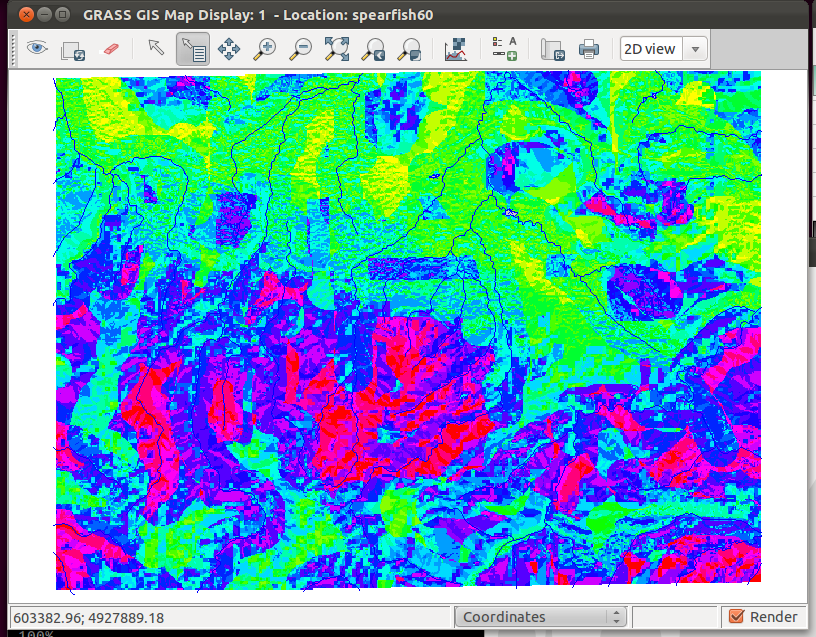
\includegraphics[scale=0.35]{grass021.png}
   %caption of the figure
   \caption{Scoring Map before masking (ref as score\_temp above)}
   %label of the figure, which has to correspond to \ref{}:
   \label{fig:grass021}
\end{figure}

\subsection{Clumping Suitable Areas}
WARNING: This part of the Laboratory involves the use of the command line (command prompt).

What is ``clumping''?
Recategorizes data in a raster map layer by grouping cells that form physically discrete areas into unique categories.

Now find the discrete areas (clumps) of aggregated habitat scores.
Run \textit{r.clump (..=>Clump Small Areas) }on the ``\textit{class}'' map to give each clump its own category number. You may call the output ``\textit{class\_clumped}''.

\begin{smallverbatim}
r.clump input=score_final_clean
 output=score_clumped
\end{smallverbatim}

Display your newly clumped map ``\textit{score\_clumped}''. It should somewhat look like this one:Fig.~\ref{fig:grass022}

%\setkeys{Gin}{width=1\textwidth}
\begin{figure}[htbp]
   \centering
   %name of your graphic, without the path AND in PNG (screnshots etc)/PDF (drawings) format:
   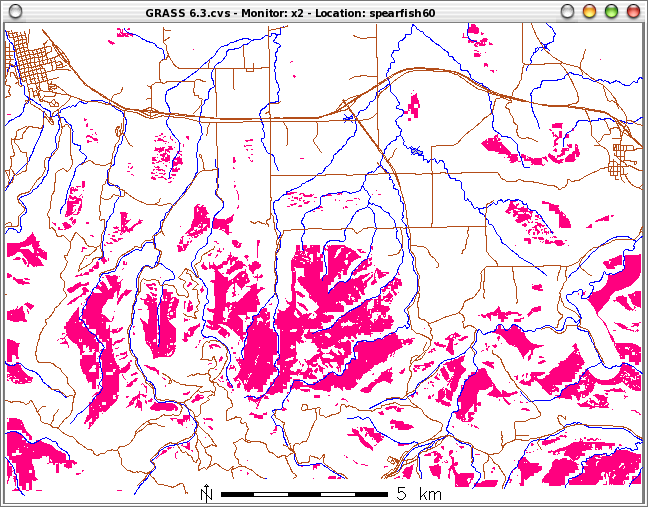
\includegraphics[scale=0.35]{grass022.png}
   %caption of the figure
   \caption{Clumped map}
   %label of the figure, which has to correspond to \ref{}:
   \label{fig:grass022}
\end{figure}


Since this species is most viable in larger clumps, extract the clumps greater than 50 hectares to a separate map. You may use the command line for reclassification by area threshold to select area superior to 50 hectares:

\begin{smallverbatim}
r.reclass.area input=score_clumped
 output=habitat_area greater=50
\end{smallverbatim}

Output ``habitat\_area'' at this level should be similar to this one:Fig.~\ref{fig:grass023}

%\setkeys{Gin}{width=1\textwidth}
\begin{figure}[htbp]
   \centering
   %name of your graphic, without the path AND in PNG (screnshots etc)/PDF (drawings) format:
   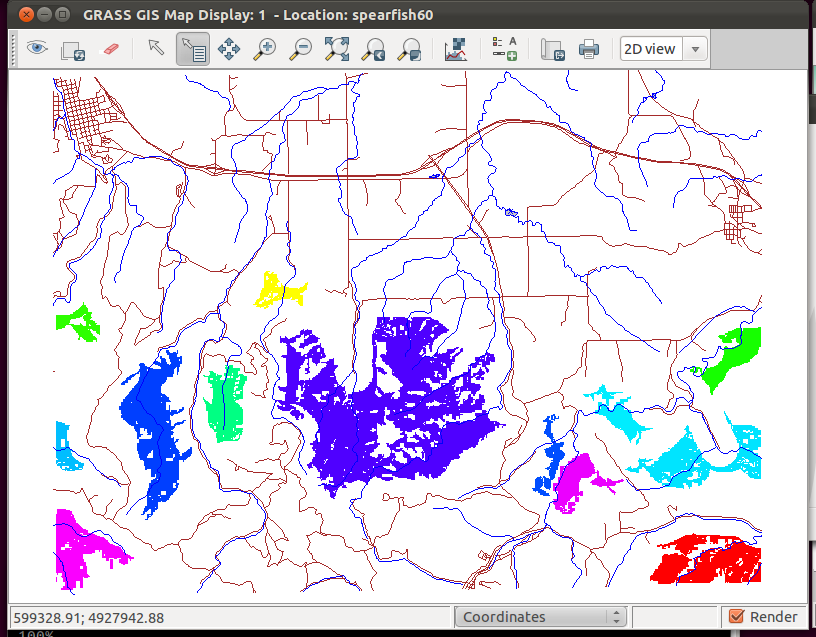
\includegraphics[scale=0.35]{grass023.png}
   %caption of the figure
   \caption{Selected Habitat Areas}
   %label of the figure, which has to correspond to \ref{}:
   \label{fig:grass023}
\end{figure}

\subsection{Export Shapefile}
Since the users work in vector GIS, we are going to convert the results in vector format and export them from GRASS GIS to shapefile.

\begin{smallverbatim}
r.to.vect -s --overwrite input=habitat_area
 output=habitat_area feature=area
\end{smallverbatim}

Vectorize the habitat\_area map you just produced (\textbf{File/Map type conversion/raster to vector}) and check that you have effectively created a polygon vector map by displaying your vector using random colors.Fig.~\ref{fig:grass024}

%\setkeys{Gin}{width=1\textwidth}
\begin{figure}[htbp]
   \centering
   %name of your graphic, without the path AND in PNG (screnshots etc)/PDF (drawings) format:
   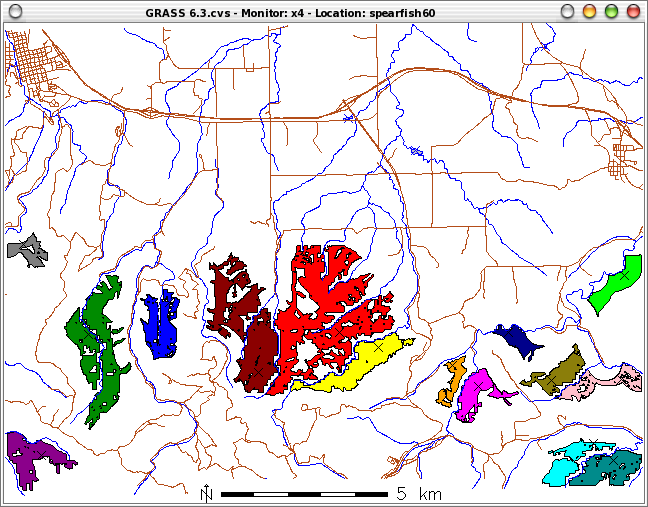
\includegraphics[scale=0.35]{grass024.png}
   %caption of the figure
   \caption{Vector Export}
   %label of the figure, which has to correspond to \ref{}:
   \label{fig:grass024}
\end{figure}

Export this selected habitat vector file along with the ``\textit{roads}'' and ``\textit{streams}'' vector files into shapefile. Please be sure that you export the same type of vectors (areas for ``\textit{habitat\_area}'' and lines for ``\textit{roads}'' and ``\textit{streams}''). Display and query them using Quantum GIS.

\begin{smallverbatim}
v.out.ogr -c input=habitat_area type=area
 dsn=QGISDATA layer=1 format=ESRI_Shapefile

v.out.ogr input=roads type=line dsn=QGISDATA
 layer=1 format=ESRI_Shapefile

v.out.ogr input=streams type=line dsn=QGISDATA
 layer=1 format=ESRI_Shapefile
\end{smallverbatim}

Additional processing.....

The pickled strumpet is quite intolerant of edge disturbances, so you would like to weight interior areas of the habitat clumps more highly than edge areas. Create interior 100-meter-interval buffers within the large habitat clumps, where interior pixels within 100 meters of a clump edge have a weight of 1, interior pixels 100-200 meters from a clump edge have a weight of 2, interior pixels 200-300 meters from a clump edge have a weight of 3, etc., and pixels outside the largest clumps have a weight of zero.

Use \textit{r.mapcalc} to multiply the aggregate habitat score map by these interior buffer weights.
Now run \textit{r.volume }on this buffer-weighted habitat score map to obtain the sum and average of each clump s cell habitat scores.
Use \textit{awk} to create reclass rules files, then use \textit{r.reclass} to map the largest clumps by sum and average habitat scores.
Which clump has the highest weighted total habitat score? Which has the highest weighted average habitat score?
Use \textit{r.grow} to create a map of clump edges only (subtracting the input map from the output map).
Use the edge map to index the perimeter of each of the major clumps.
Calculate the compactness (area divided by perimeter squared) of each clump.
Map the largest clumps by compactness. Create a jazzy display script to demonstrate your procedures and explain your findings.
(See \href{http://www.udel.edu/johnmack/frec682/script_ideas.html})

A script for some parts of the Lab is in \textbf{Appendix B} \ref{appendixB}.

\newpage
\section{Remote sensing}
\label{remote_sensing}

\subsection{Import}
\label{Import}

Download from GLCF website a satellite image of Landsat 7 ETM+ covering your country, or area of interest. In this case it is p092r084 from year 2010 and Julian day 26, it is in the South-East Australia. We took a small geographical sample by this gdal shell script:

\begin{smallverbatim}
 #Uncompress the tarball
 tar xvf LE70920842010026ASN00.tar.gz
 cd LE70920842010026ASN00/

 #subset all Landsat 7 bands
 for file in *.TIF
   do gdalwarp -te 452274 -3855746 476447
      -3839082 $file new$file
   #remove quietly the $file
   rm -f $file
 done
\end{smallverbatim}


Start GRASS GIS. On opening, click on ``Location Wizard'', set your Location name, press ``Next'', then click on the third option ``Read projection and datum terms for a georeferenced data file'' button and select one of the Landsat TIF files. Then agree to all until completion.

%\setkeys{Gin}{width=1\textwidth}
\begin{figure}[htbp]
   \centering
   %name of your graphic, without the path AND in PNG (screnshots etc)/PDF (drawings) format:
   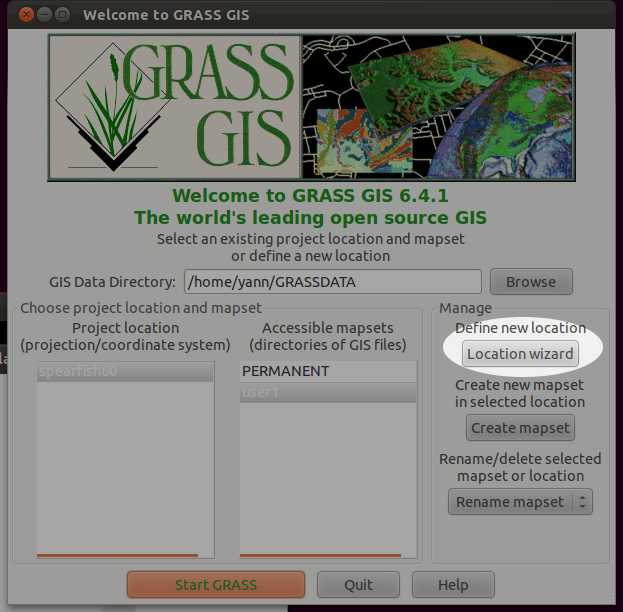
\includegraphics[scale=0.35]{grass_rs000.png}
   %caption of the figure
   \caption{Start GRASS GIS}
   %label of the figure, which has to correspond to \ref{}:
   \label{fig:grass_rs000}
\end{figure}

On launching the module, type in ``landsat'' or whatever name you created and load your landsat images into it.

%\setkeys{Gin}{width=1\textwidth}
\begin{figure}[htbp]
   \centering
   %name of your graphic, without the path AND in PNG (screnshots etc)/PDF (drawings) format:
   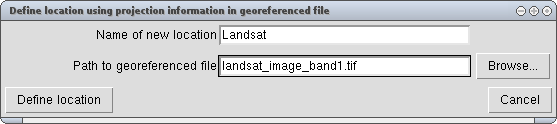
\includegraphics[scale=0.35]{grass_rs001.png}
   %caption of the figure
   \caption{Set up the new Location name}
   %label of the figure, which has to correspond to \ref{}:
   \label{fig:grass_rs001}
\end{figure}

Once setup from georeferenced file, launch GRASS GIS from this new Location called ''landsat''.

Identify with band number corresponding to which spectrum band, especially Red and Near-InfraRed spectra.

Once GRASS is loaded, import in GRASS GIS using r.in.gdal (File / import raster data / Common import formats).

%\setkeys{Gin}{width=1\textwidth}
\begin{figure}[htbp]
   \centering
   %name of your graphic, without the path AND in PNG (screnshots etc)/PDF (drawings) format:
   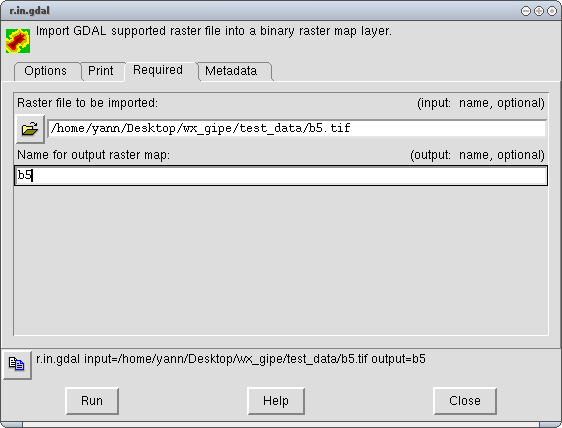
\includegraphics[scale=0.35]{grass_rs002.png}
   %caption of the figure
   \caption{import with r.in.gdal}
   %label of the figure, which has to correspond to \ref{}:
   \label{fig:grass_rs002}
\end{figure}

Change the coloring of the bands R=3, G=2 and B=1 according to r.landsat.rgb:

%\setkeys{Gin}{width=1\textwidth}
\begin{figure}[htbp]
   \centering
   %name of your graphic, without the path AND in PNG (screnshots etc)/PDF (drawings) format:
   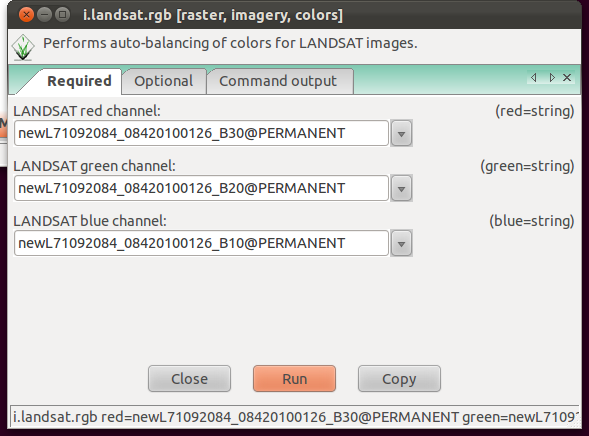
\includegraphics[scale=0.35]{grass_rs003.png}
   %caption of the figure
   \caption{Change RGB color table for Landsat}
   %label of the figure, which has to correspond to \ref{}:
   \label{fig:grass_rs003}
\end{figure}

Load a RGB combination of band 4,3,2 by clicking the 8th button from the left near to th raster loading button, select there the RGB map.

%\setkeys{Gin}{width=1\textwidth}
\begin{figure}[htbp]
   \centering
   %name of your graphic, without the path AND in PNG (screnshots etc)/PDF (drawings) format:
   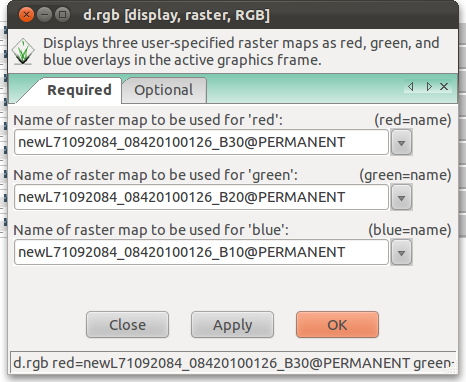
\includegraphics[scale=0.45]{grass_rs004.png}
   %caption of the figure
   \caption{Load a RGB band combination}
   %label of the figure, which has to correspond to \ref{}:
   \label{fig:grass_rs004}
\end{figure}

Display the map (real color composite)

%\setkeys{Gin}{width=1\textwidth}
\begin{figure}[htbp]
   \centering
   %name of your graphic, without the path AND in PNG (screnshots etc)/PDF (drawings) format:
   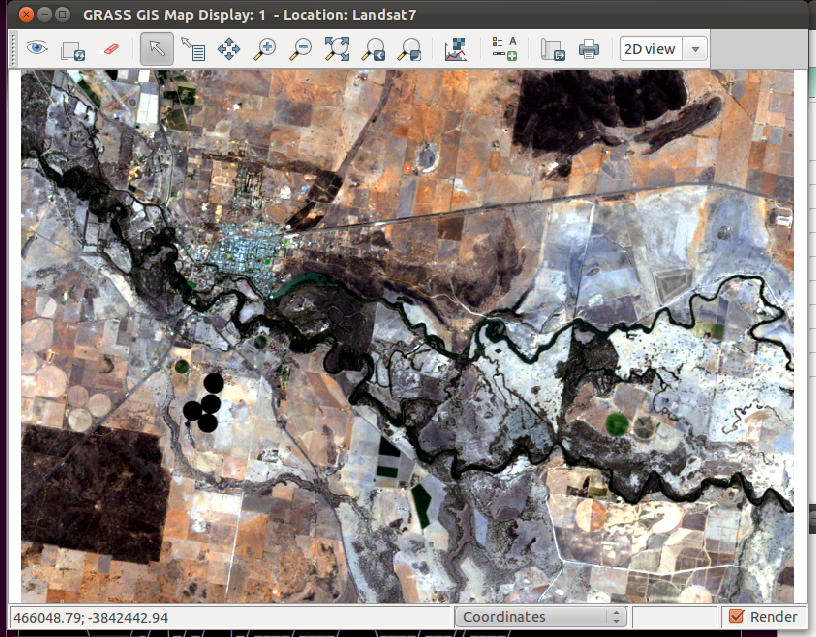
\includegraphics[scale=0.35]{grass_rs005.png}
   %caption of the figure
   \caption{Display the RGB real colour composite}
   %label of the figure, which has to correspond to \ref{}:
   \label{fig:grass_rs005}
\end{figure}

Change the coloring of the bands according to this (False Colour Composite).

%\setkeys{Gin}{width=1\textwidth}
\begin{figure}[htbp]
   \centering
   %name of your graphic, without the path AND in PNG (screnshots etc)/PDF (drawings) format:
   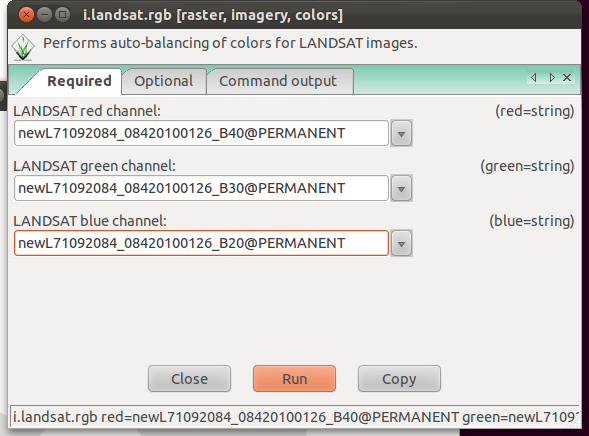
\includegraphics[scale=0.35]{grass_rs006.png}
   %caption of the figure
   \caption{Load NIR-R-B colour combination)}
   %label of the figure, which has to correspond to \ref{}:
   \label{fig:grass_rs006}
\end{figure}

Display the map of the false color composite

%\setkeys{Gin}{width=1\textwidth}
\begin{figure}[htbp]
   \centering
   %name of your graphic, without the path AND in PNG (screnshots etc)/PDF (drawings) format:
   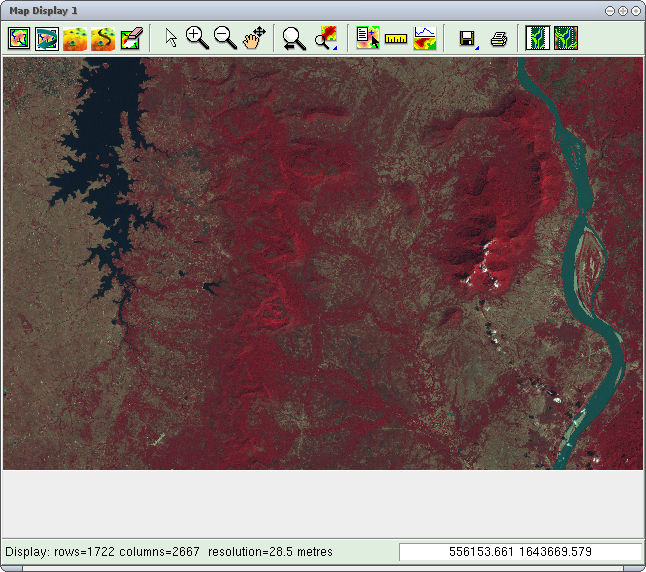
\includegraphics[scale=0.35]{grass_rs007.png}
   %caption of the figure
   \caption{Display the RGB FCC}
   %label of the figure, which has to correspond to \ref{}:
   \label{fig:grass_rs007}
\end{figure}

\subsection{Classification}
\label{classification}

Create a group and subgroup with band 1-5.

%\setkeys{Gin}{width=1\textwidth}
\begin{figure}[htbp]
   \centering
   %name of your graphic, without the path AND in PNG (screnshots etc)/PDF (drawings) format:
   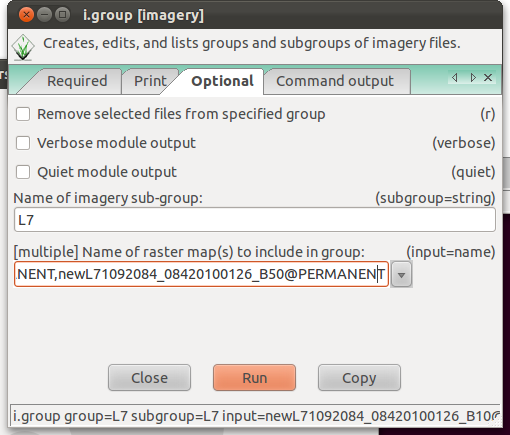
\includegraphics[scale=0.45]{grass_rs008.png}
   %caption of the figure
   \caption{Create image group and subgroup}
   %label of the figure, which has to correspond to \ref{}:
   \label{fig:grass_rs008}
\end{figure}

Create a signature file.

%\setkeys{Gin}{width=1\textwidth}
\begin{figure}[htbp]
   \centering
   %name of your graphic, without the path AND in PNG (screnshots etc)/PDF (drawings) format:
   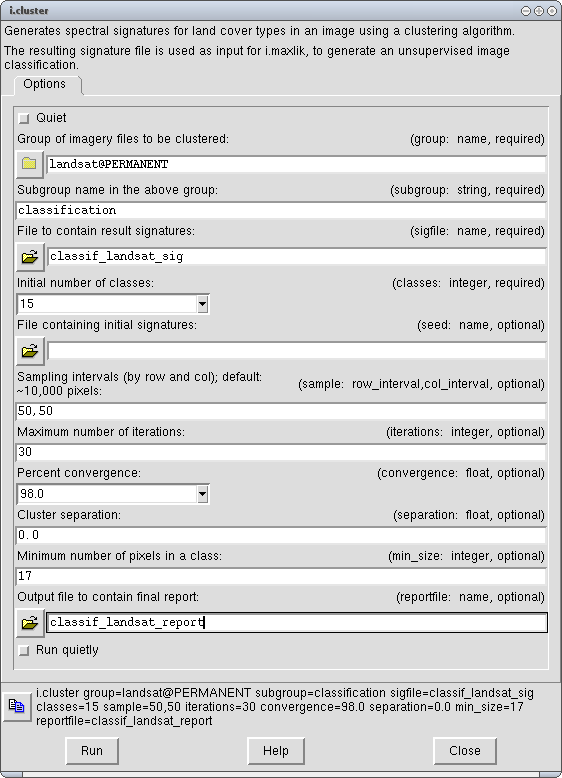
\includegraphics[scale=0.35]{grass_rs009.png}
   %caption of the figure
   \caption{Create initial class statistics signature file}
   %label of the figure, which has to correspond to \ref{}:
   \label{fig:grass_rs009}
\end{figure}

See the convergence happening...

%\setkeys{Gin}{width=1\textwidth}
\begin{figure}[htbp]
   \centering
   %name of your graphic, without the path AND in PNG (screnshots etc)/PDF (drawings) format:
   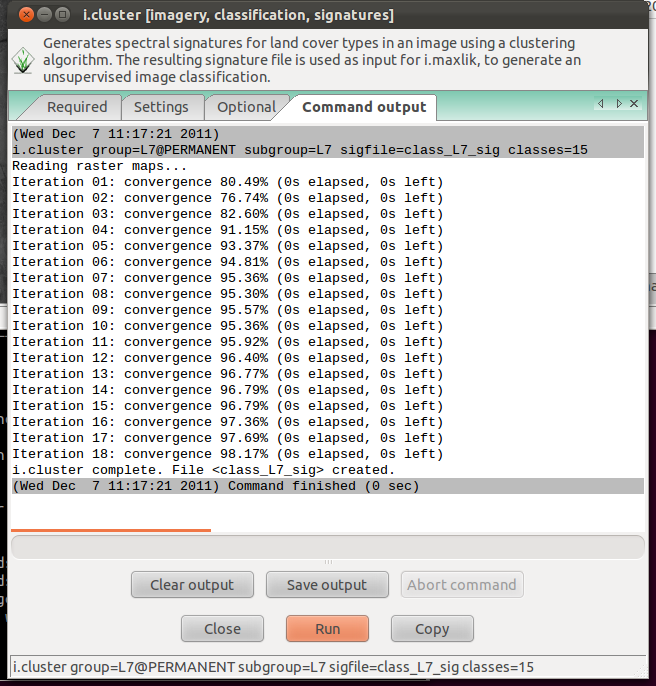
\includegraphics[scale=0.35]{grass_rs010.png}
   %caption of the figure
   \caption{Convergence of statistics}
   %label of the figure, which has to correspond to \ref{}:
   \label{fig:grass_rs010}
\end{figure}

Run the Maximum Likelihood clustering classification.

%\setkeys{Gin}{width=1\textwidth}
\begin{figure}[htbp]
   \centering
   %name of your graphic, without the path AND in PNG (screnshots etc)/PDF (drawings) format:
   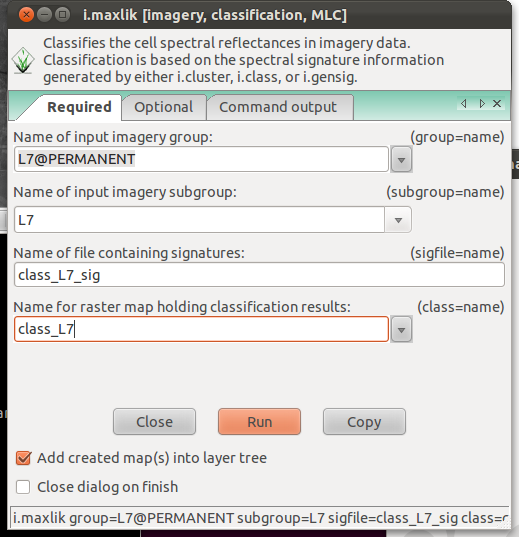
\includegraphics[scale=0.35]{grass_rs011.png}
   %caption of the figure
   \caption{Create initial class statistics signature file}
   %label of the figure, which has to correspond to \ref{}:
   \label{fig:grass_rs011}
\end{figure}

Display the result of unsupervised classification

%\setkeys{Gin}{width=1\textwidth}
\begin{figure}[htbp]
   \centering
   %name of your graphic, without the path AND in PNG (screnshots etc)/PDF (drawings) format:
   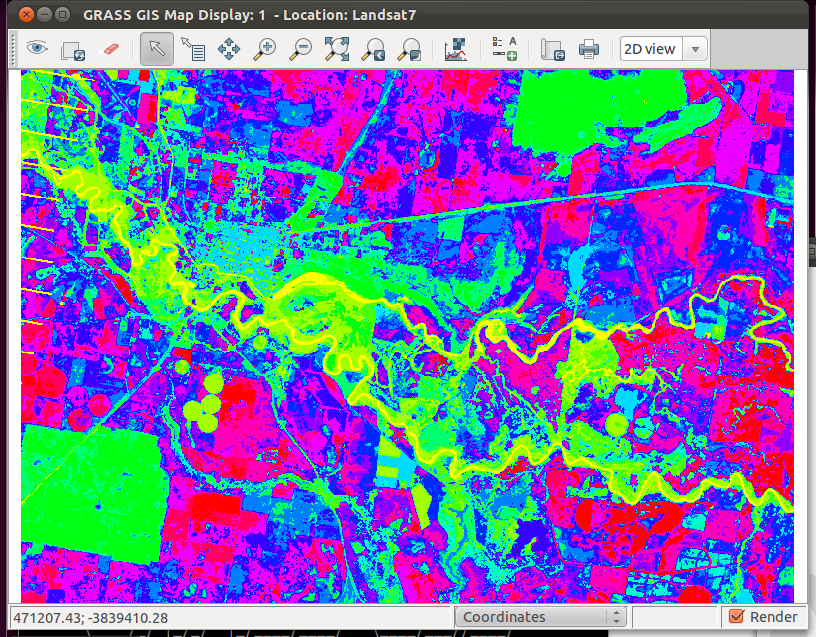
\includegraphics[scale=0.35]{grass_rs012.png}
   %caption of the figure
   \caption{Display classification result}
   %label of the figure, which has to correspond to \ref{}:
   \label{fig:grass_rs012}
\end{figure}

\subsection{Map Algebra}
\label{map_algebra}

Using r.mapcalc, calculate the difference vegetation index (dvi), the Normalized dvi (ndvi) and the soil-adjusted vegetation index (savi). Then calculate some uncorrected Albedo and the temperature.

\begin{enumerate}
 \item dvi=(NIR-RED)
 \item ndvi=dvi/(NIR+RED)
 \item savi=((1+0.5)*dvi)/(NIR+RED+0.5)
 \item Albedo=0.293*BLUE + 0.274*GREEN + 0.233*RED + 0.156*NIR + 0.033*band5 +0.011*band7
 \item temperature=1282.71 / (log ((666.09 / (band6)) + 1.0))
\end{enumerate}

Observe cities, roads, irrigation canals, rivers, wetlands, agricultural lands, forests and barren areas with each and all of these images, find out what defines best each land use.

\newpage
\section{3D Visualization}
\label{3D_visualization}


The N-Visualization tool in GRASS GIS takes care of 3D display of GIS data. Identify the 3 N-VIZ buttons in the GRASS GIS GUI. Click on the Left Side button. This will launch NVIZ.

%\setkeys{Gin}{width=1\textwidth}
\begin{figure}[htbp]
   \centering
   %name of your graphic, without the path AND in PNG (screnshots etc)/PDF (drawings) format:
   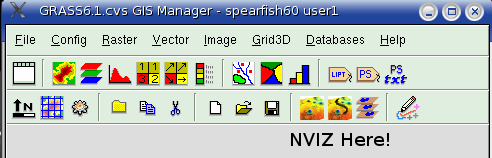
\includegraphics[scale=0.35]{nviz000.png}
   %caption of the figure
   \caption{Find out the 3 NVIZ buttons}
   %label of the figure, which has to correspond to \ref{}:
   \label{fig:nviz000}
\end{figure}


%\setkeys{Gin}{width=1\textwidth}
\begin{figure}[htbp]
   \centering
   %name of your graphic, without the path AND in PNG (screnshots etc)/PDF (drawings) format:
   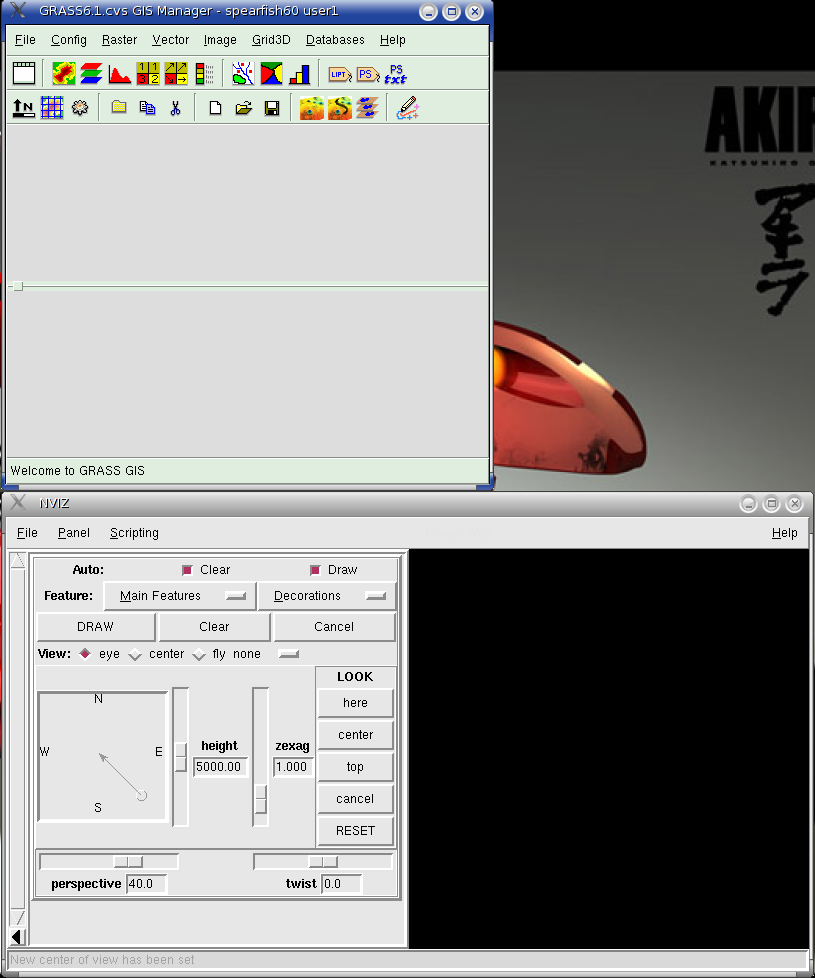
\includegraphics[scale=0.2]{nviz001.png}
   %caption of the figure
   \caption{NVIZ Display}
   %label of the figure, which has to correspond to \ref{}:
   \label{fig:nviz001}
\end{figure}

Open the Panel and detach it.

%\setkeys{Gin}{width=1\textwidth}
\begin{figure}[htbp]
   \centering
   %name of your graphic, without the path AND in PNG (screnshots etc)/PDF (drawings) format:
   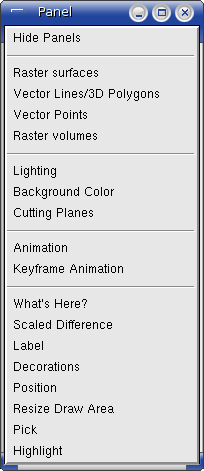
\includegraphics[scale=0.35]{nviz002.png}
   %caption of the figure
   \caption{NVIZ panel detached}
   %label of the figure, which has to correspond to \ref{}:
   \label{fig:nviz002}
\end{figure}

Load a Raster by clicking on Raster surfaces

%\setkeys{Gin}{width=1\textwidth}
\begin{figure}[htbp]
   \centering
   %name of your graphic, without the path AND in PNG (screnshots etc)/PDF (drawings) format:
   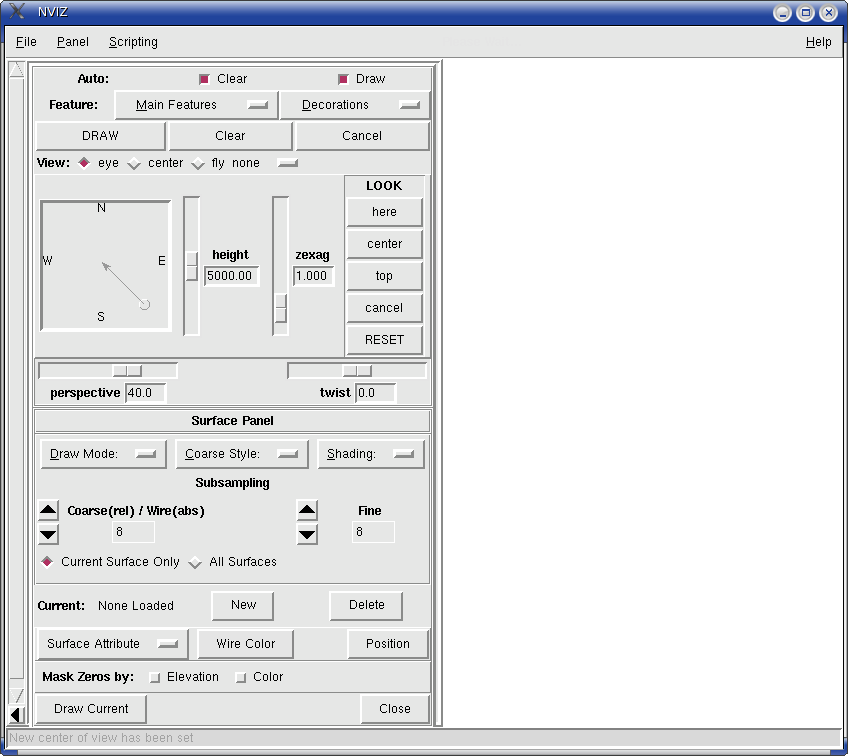
\includegraphics[scale=0.2]{nviz003.png}
   %caption of the figure
   \caption{Load a raster}
   %label of the figure, which has to correspond to \ref{}:
   \label{fig:nviz003}
\end{figure}

In the Surface Panel, click on the NEW button,select NEW MAP.

%\setkeys{Gin}{width=1\textwidth}
\begin{figure}[htbp]
   \centering
   %name of your graphic, without the path AND in PNG (screnshots etc)/PDF (drawings) format:
   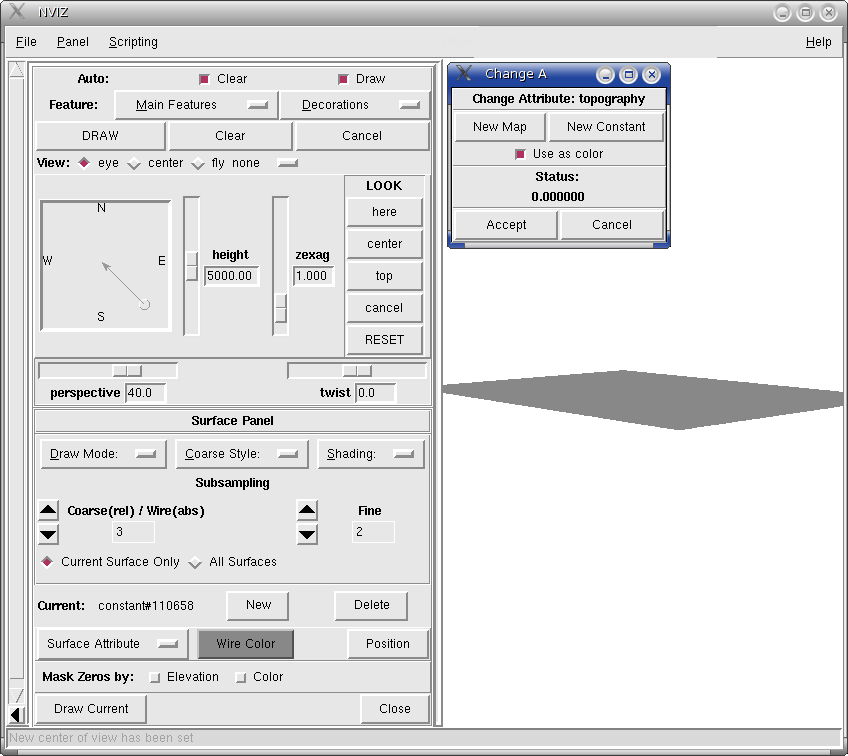
\includegraphics[scale=0.2]{nviz004.png}
   %caption of the figure
   \caption{Select New Map}
   %label of the figure, which has to correspond to \ref{}:
   \label{fig:nviz004}
\end{figure}

This will load a mapset locator, select permanent, then in the coverage browser select elevation.10m.

%\setkeys{Gin}{width=1\textwidth}
\begin{figure}[htbp]
   \centering
   %name of your graphic, without the path AND in PNG (screnshots etc)/PDF (drawings) format:
   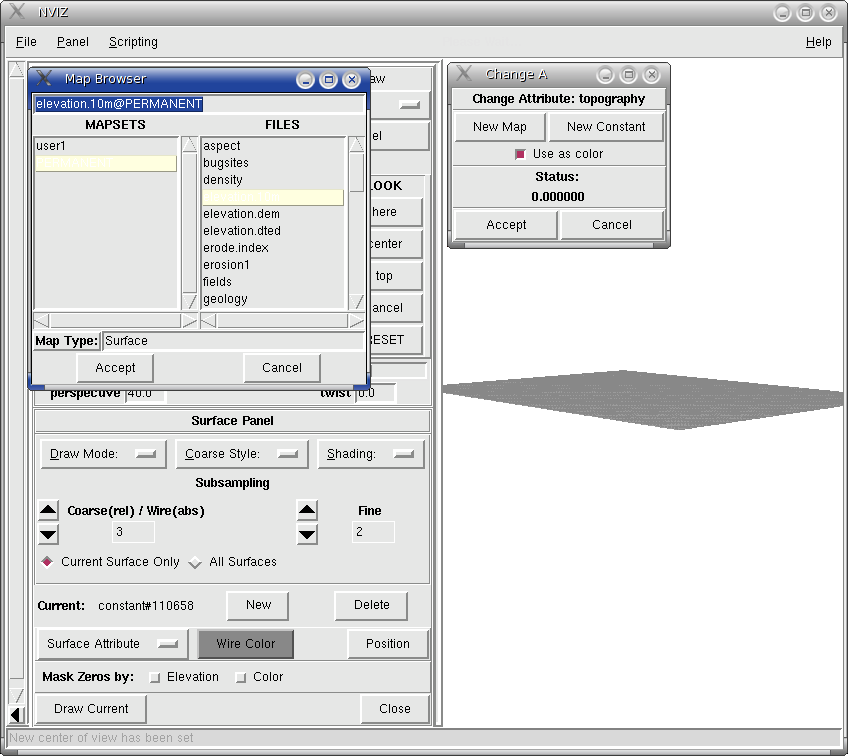
\includegraphics[scale=0.2]{nviz005.png}
   %caption of the figure
   \caption{Select elevation.10m}
   %label of the figure, which has to correspond to \ref{}:
   \label{fig:nviz005}
\end{figure}

Accept for each open dialog. The raster will be loaded.

%\setkeys{Gin}{width=1\textwidth}
\begin{figure}[htbp]
   \centering
   %name of your graphic, without the path AND in PNG (screnshots etc)/PDF (drawings) format:
   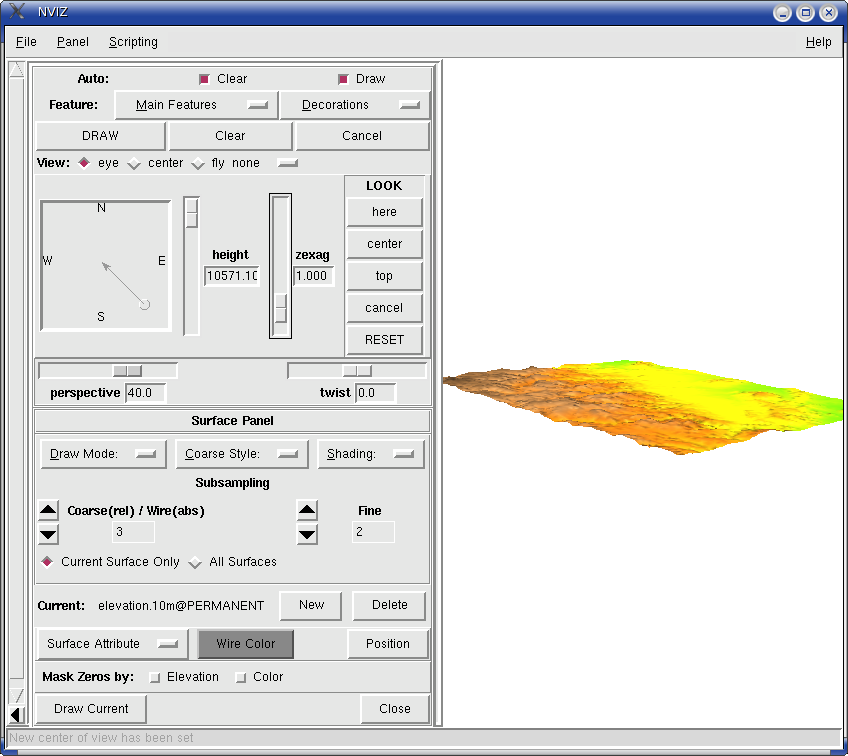
\includegraphics[scale=0.2]{nviz006.png}
   %caption of the figure
   \caption{Load elevation.10m}
   %label of the figure, which has to correspond to \ref{}:
   \label{fig:nviz006}
\end{figure}

Close the Surface Panel and Open the Vector Panel.

%\setkeys{Gin}{width=1\textwidth}
\begin{figure}[htbp]
   \centering
   %name of your graphic, without the path AND in PNG (screnshots etc)/PDF (drawings) format:
   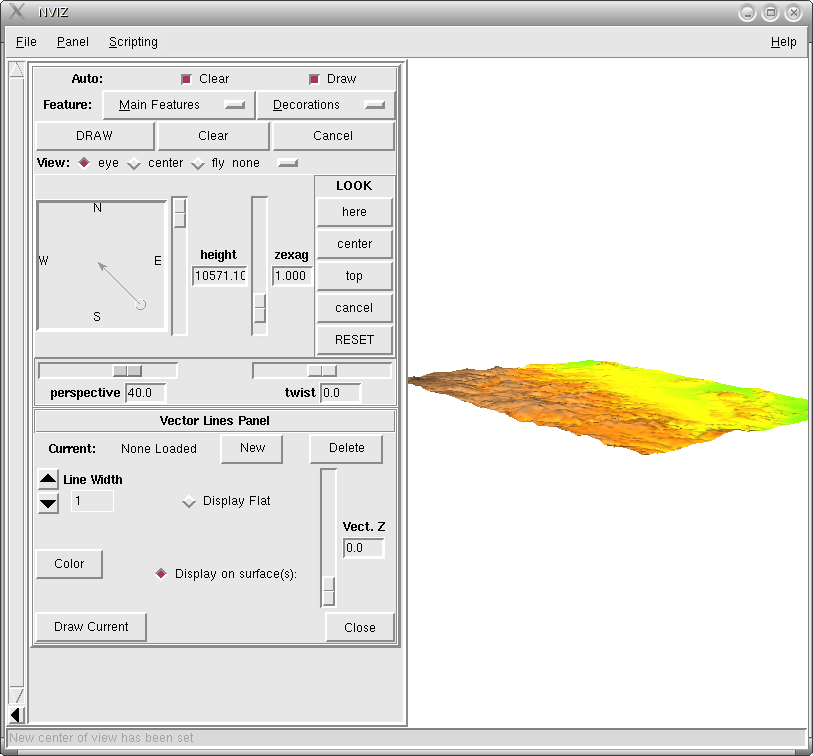
\includegraphics[scale=0.2]{nviz007.png}
   %caption of the figure
   \caption{Open Vector Panel}
   %label of the figure, which has to correspond to \ref{}:
   \label{fig:nviz007}
\end{figure}

Select NEW. This will open the mapset browser again, choose PERMANENT, select streams coverage.

%\setkeys{Gin}{width=1\textwidth}
\begin{figure}[htbp]
   \centering
   %name of your graphic, without the path AND in PNG (screnshots etc)/PDF (drawings) format:
   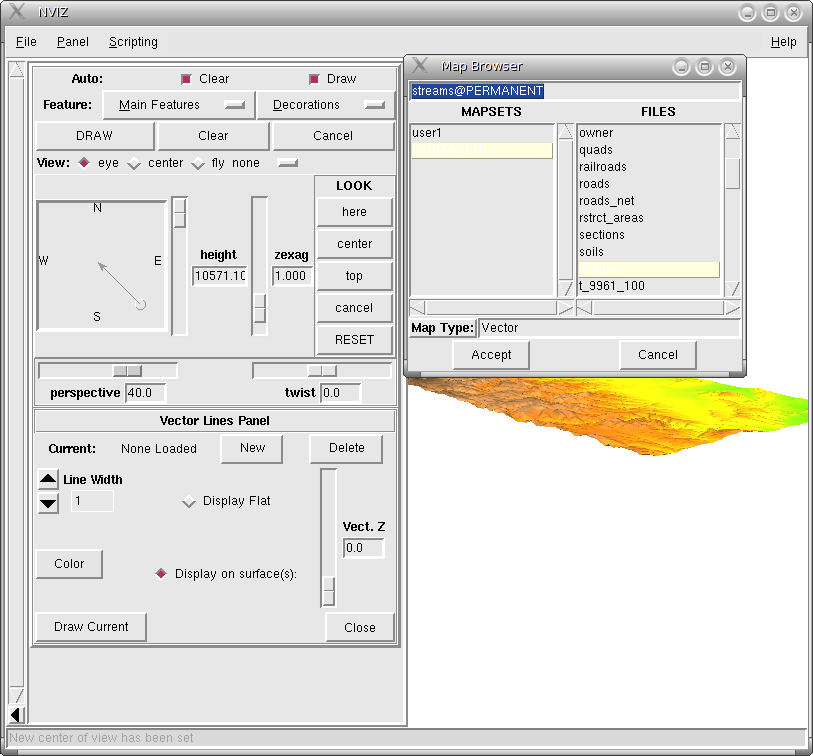
\includegraphics[scale=0.2]{nviz008.png}
   %caption of the figure
   \caption{Load Streams vector layer}
   %label of the figure, which has to correspond to \ref{}:
   \label{fig:nviz008}
\end{figure}

Accept and click the button called DRAW CURRENT.

%\setkeys{Gin}{width=1\textwidth}
\begin{figure}[htbp]
   \centering
   %name of your graphic, without the path AND in PNG (screnshots etc)/PDF (drawings) format:
   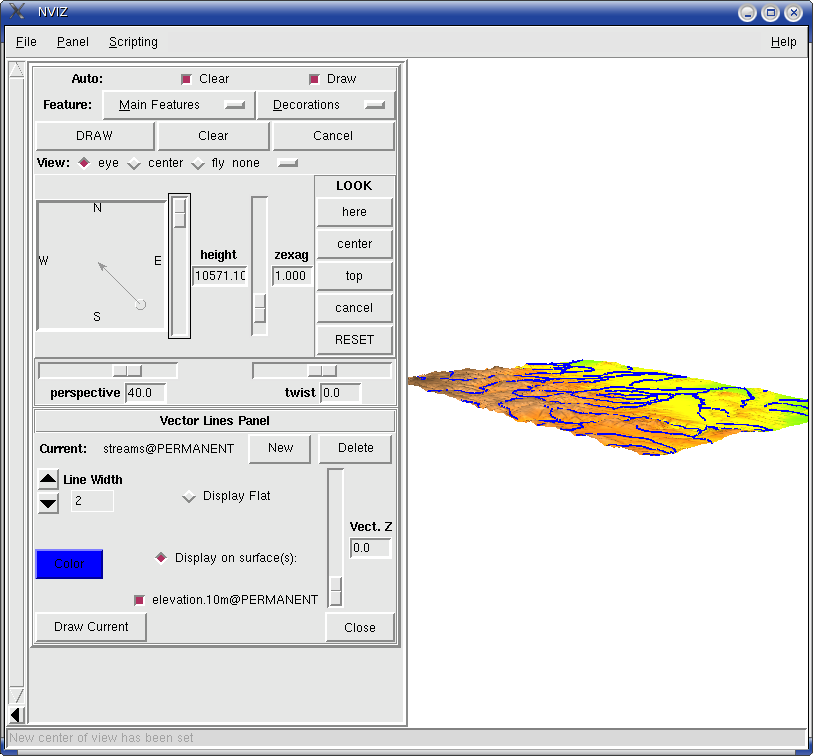
\includegraphics[scale=0.2]{nviz009.png}
   %caption of the figure
   \caption{Draw Streams Layer}
   %label of the figure, which has to correspond to \ref{}:
   \label{fig:nviz009}
\end{figure}

Close the vector panel and open the color panel from the main panel.

%\setkeys{Gin}{width=1\textwidth}
\begin{figure}[htbp]
   \centering
   %name of your graphic, without the path AND in PNG (screnshots etc)/PDF (drawings) format:
   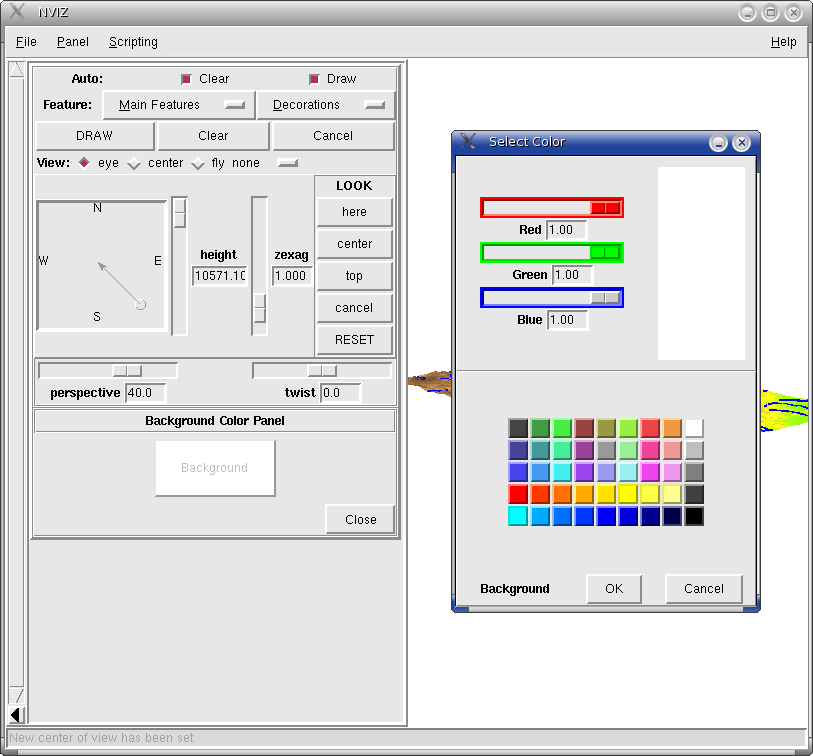
\includegraphics[scale=0.2]{nviz010.png}
   %caption of the figure
   \caption{Open color panel}
   %label of the figure, which has to correspond to \ref{}:
   \label{fig:nviz010}
\end{figure}

Select your color and CLOSE the color panel.

%\setkeys{Gin}{width=1\textwidth}
\begin{figure}[htbp]
   \centering
   %name of your graphic, without the path AND in PNG (screnshots etc)/PDF (drawings) format:
   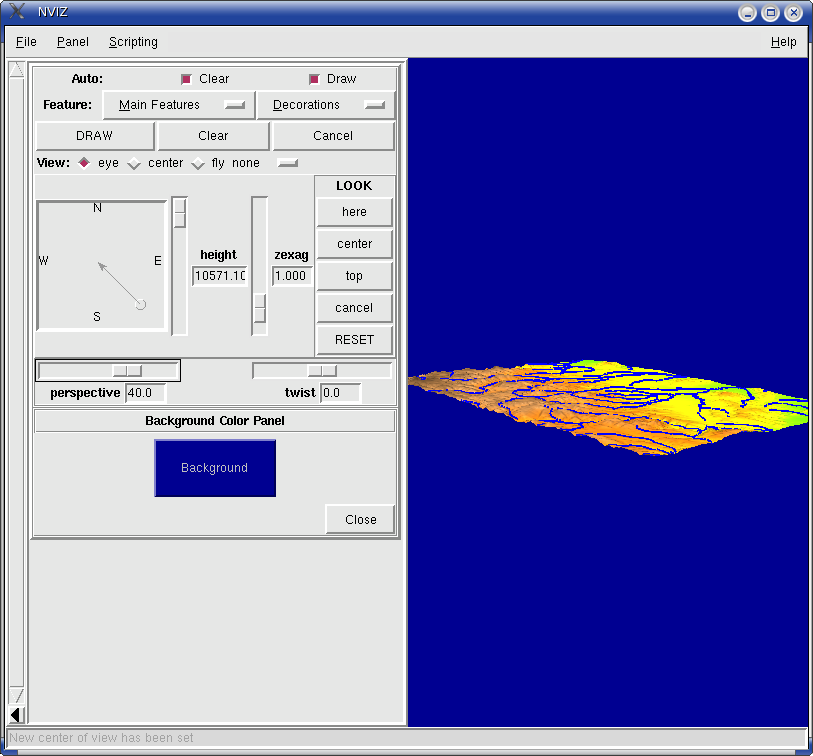
\includegraphics[scale=0.2]{nviz011.png}
   %caption of the figure
   \caption{Select your color}
   %label of the figure, which has to correspond to \ref{}:
   \label{fig:nviz011}
\end{figure}

Drag the directional ball-point to the Upper-left, closer to the center. Increase Height exaggeration to 3.0.

%\setkeys{Gin}{width=1\textwidth}
\begin{figure}[htbp]
   \centering
   %name of your graphic, without the path AND in PNG (screnshots etc)/PDF (drawings) format:
   \includegraphics[scale=0.2]{nviz012.png}
   %caption of the figure
   \caption{Change the z-exaggeration and camera settings}
   %label of the figure, which has to correspond to \ref{}:
   \label{fig:nviz012}
\end{figure}

\newpage
\subsection{Appendix A: Overview of Grass GUI}
\label{appendixA}

Overview of the available commands in the modules:Fig.~\ref{fig:grass025} Fig.~\ref{fig:grass026} Fig.~\ref{fig:grass027}

%\setkeys{Gin}{width=1\textwidth}
\begin{figure}[htbp]
   \centering
   %name of your graphic, without the path AND in PNG (screnshots etc)/PDF (drawings) format:
   \includegraphics[scale=0.4]{grass025.png}
   %caption of the figure
   \caption{GRASS Menus (1/3)}
   %label of the figure, which has to correspond to \ref{}:
   \label{fig:grass025}
\end{figure}

%\setkeys{Gin}{width=1\textwidth}
\begin{figure}[htbp]
   \centering
   %name of your graphic, without the path AND in PNG (screnshots etc)/PDF (drawings) format:
   \includegraphics[scale=0.4]{grass026.png}
   %caption of the figure
   \caption{GRASS Menus (2/3)}
   %label of the figure, which has to correspond to \ref{}:
   \label{fig:grass026}
\end{figure}

%\setkeys{Gin}{width=1\textwidth}
\begin{figure}[htbp]
   \centering
   %name of your graphic, without the path AND in PNG (screnshots etc)/PDF (drawings) format:
   \includegraphics[scale=0.4]{grass027.png}
   %caption of the figure
   \caption{GRASS Menus (3/3)}
   %label of the figure, which has to correspond to \ref{}:
   \label{fig:grass027}
\end{figure}

\newpage

\subsection{Appendix B: GRASS SCRIPT}
\label{appendixB}

Please put this into a file that you may name \textit{script.sh}\textup{and from a }\textit{Terminal}\textup{ type: ``chmod 0755}\textit{script.sh''}\textup{. Then you can run the script }by typing the command: ``./script.sh''.

\begin{smallverbatim}
#!/bin/bash
# main map names variables
dem=elevation.dem
r=roads
s=streams
# buffer streams and roads variables
_bs=_bstreams500
_br=_broads500
# reclassed buffer streams and roads variables
_rbs=_rbstreams500
_rbr=_rbroads500
#--------------------------------------------------
# General Presentation: Start Monitor 0
#--------------------------------------------------
d.mon start=x0
d.erase color=grey
d.rast map=\$dem
sleep 1
d.vect map=\$r color=brown
sleep 1
d.vect map=\$s color=blue
sleep 1
d.barscale bcolor=white tcolor=black at=30.0,95.0
sleep 2
#--------------------------------------------------
# Buffering: Start Monitor 1
#--------------------------------------------------
d.mon start=x1
d.mon select=x1
d.erase color=grey
r.buffer input=\$s output=\$_bs distances=500
 units=meters --overwrite
r.null map=\$_bs null=0
d.rast map=\$_bs
d.vect map=\$s color=blue
d.barscale bcolor=white tcolor=black at=30.0,95.0
r.buffer input=\$r output=\$_br distances=500
 units=meters --overwrite
r.null map=\$_br null=0
d.rast map=\$_br
d.vect map=\$s color=blue
d.barscale bcolor=white tcolor=black at=30.0,95.0
#--------------------------------------------------
# Reclassification: Start Monitor 2
#--------------------------------------------------
d.mon start=x2
d.mon select=x2
d.erase color=grey
echo "...Reclassify..."
r.mapcalc \$_rbs="if(\$_bs==2,1,0)"
r.mapcalc _s_sl="if(\$_rbs==1,if(slope<=5,2,5),0)"
r.mapcalc \$_rbr="float(if(\$_br==2,-5.0,0))"
r.mapcalc _for="if(vegcover==3,4,0)"
r.mapcalc _for1="if(vegcover==5,1,0)"
r.mapcalc _exp1="if(aspect<45.0 || aspect>314.0 &&
 aspect != 0.0,1,0)"
r.mapcalc _exp2="if(aspect<225.0 && aspect>135.
 0,1,0)"
r.mapcalc _exp3="if(aspect<=135.0 && aspect>=45.0,
 3,0)"
r.mapcalc _elev1="if(\$dem<1400 &&\$dem>1200,2,0)"
r.mapcalc _elev2="if(\$dem<1600 &&\$dem>=1400,4,0)"
r.mapcalc _elev3="if(\$dem>=1600,2,0)"
#--------------------------------------------------
r.buffer input=\$r output=_br100 distances=100
 units=meters --overwrite
r.null map=\_br100 null=0
r.mapcalc _add="float(_s_sl+\$_rbr+_for+_for1+
 _exp1+_exp2+_exp3+_elev1+_elev2+_elev3)"
r.mapcalc _clas="if(_add{>9,1,null())"
r.mapcalc _class="if(_clas==1&&_br100==0,1,null())"
echo "Reclassification...done."
d.rast map="\$_rbs"
sleep 1
d.rast map="_s_sl"
d.rast map="\$_rbr"
d.rast map="_for"
d.rast map="_for1"
d.rast map="_exp1"
d.rast map="_exp2"
d.rast map="_exp3"
d.rast map="_elev1"
d.rast map="_elev2"
d.rast map="_elev3"
d.rast map="_br100"
sleep 1
#r.colors color=grey map="_add"
d.rast map="_add"
sleep 1
d.rast map="_class"
sleep 1
#d.erase
d.vect map="\$s" color=blue
d.vect map="\$r" color=brown
d.barscale bcolor=white tcolor=black at=30.0,95.0
sleep 5
g.remove
rast="\$_rbs,_s_sl,\$_rbr,_for,_for1"}
g.remove
rast="_exp1,_exp2,_exp3,_elev1"}
g.remove
rast="_elev2,_elev3,_br100,_add"}
g.remove rast="\$_bs,\$_br,_clas"}
sleep 1
echo ""
echo "finished"
sleep 1
#--------------------------------------------------
# Clumping: Start Monitor 3
#--------------------------------------------------
d.mon start=x3
d.mon select=x3
d.erase color=grey
g.remove rast=_clump.clump._rclumpnew
r.clump input=_class output=_clump --overwrite
r.colors color=gyr map="_clump"
d.rast map="_clump"
sleep 1
r.reclass.area input=_clump greater=50
 output=_rclumpnew --overwrite
r.colors color=gyr map="_rclumpnew"
d.erase color=white
d.rast map="_rclumpnew"
sleep 1
d.vect map="streams" color=blue
d.vect map="roads" color=brown
d.barscale bcolor=white tcolor=black at=30.0,95.0
sleep 1
g.remove rast="_clump,_class"
#--------------------------------------------------
# R2V and Export: Start Monitor 4
#--------------------------------------------------
d.mon start=x4
d.mon select=x4
d.erase color=white
r.to.vect -s input=_rclumpnew output=rclump
 feature=area --overwrite
d.vect -c map=rclump type=area color=black
d.vect map="streams" color=blue
d.vect map="roads" color=brown
d.barscale bcolor=white tcolor=black at=30.0,95.0
sleep 1
v.out.ogr input=rclump type=area dsn=QGISDATA
 layer=1 format=ESRI_Shapefile --overwrite
g.remove rast="_rclumpnew"
g.remove vect="rclump"
d.mon stop=x4
d.mon stop=x3
d.mon stop=x2
d.mon stop=x1
d.mon stop=x0
\end{smallverbatim}

\address{GRASS Development Team\\
  \url{http://grass.osgeo.org}\\
  \email{grass-web@lists.osgeo.org}}

%%% Local Variables:
%%% mode: latex
%%% TeX-master: main_document.tex
%%% End:

